%%%%%%%%%%%%%%%%%%%%%%%%%%%%%%%
%This is the article LaTeX template for RSC journals
%Copyright The Royal Society of Chemistry 2010
%%%%%%%%%%%%%%%%%%%%%%%%%%%%%%%

\documentclass[8.5pt,twoside,twocolumn]{article}
\oddsidemargin -1.2cm
\evensidemargin -1.2cm
\textwidth 18cm
\headheight 1.0in
\topmargin -3.5cm
\textheight 22cm
\usepackage[super,sort&compress,comma]{natbib} 
\usepackage{mhchem}
%% \usepackage{times,mathptmx}
% \usepackage{times}
% feel free not to use mathptmx if it causes difficulties
\usepackage{sectsty}
\usepackage{balance}
\usepackage{graphicx} %eps figures can be used instead

%% \usepackage{lastpage}
%% \usepackage[format=plain,justification=raggedright,singlelinecheck=false,font=small,labelfont=bf,labelsep=space]{caption} 
\usepackage{fancyhdr}
\pagestyle{fancy}

\begin{document}

\thispagestyle{plain}
\fancypagestyle{plain}{
\fancyhead[L]{Communication}
\fancyhead[C]{\hspace{-1cm}
\includegraphics[height=20pt]{headers/CH}}
\fancyhead[R]{Science \vspace{-0.2cm}}
\renewcommand{\headrulewidth}{1pt}}
\renewcommand{\thefootnote}{\fnsymbol{footnote}}
\renewcommand\footnoterule{\vspace*{1pt}% 
\hrule width 3.4in height 0.4pt \vspace*{5pt}} 
\setcounter{secnumdepth}{5}

\makeatletter 
\def\subsubsection{\@startsection{subsubsection}{3}{10pt}{-1.25ex plus -1ex minus -.1ex}{0ex plus 0ex}{\normalsize\bf}} 
\def\paragraph{\@startsection{paragraph}{4}{10pt}{-1.25ex plus -1ex minus -.1ex}{0ex plus 0ex}{\normalsize\textit}} 
\renewcommand\@biblabel[1]{#1}            
\renewcommand\@makefntext[1]% 
{\noindent\makebox[0pt][r]{\@thefnmark\,}#1}
\makeatother 
\renewcommand{\figurename}{\small{Fig.}~}
\sectionfont{\large}
\subsectionfont{\normalsize} 

\fancyfoot{}
\fancyfoot[LO,RE]{\vspace{-7pt}Oregon State University 2017}
\fancyfoot[CO]{\vspace{-7.2pt}\hspace{12.2cm}Science}
\fancyfoot[RO]{\footnotesize{\sffamily{1--\pageref{LastPage} ~\textbar  \hspace{2pt}\thepage}}}
%% \fancyfoot[LE]{\footnotesize{\sffamily{\thepage~\textbar\hspace{3.45cm} 1--\pageref{LastPage}}}}
\fancyhead{}
\renewcommand{\headrulewidth}{1pt} 
\renewcommand{\footrulewidth}{1pt}
\setlength{\arrayrulewidth}{1pt}
\setlength{\columnsep}{6.5mm}
\setlength\bibsep{1pt}

\twocolumn[
  \begin{@twocolumnfalse}
\noindent\LARGE{\textbf{Identification of an unknown disubstituted benzene derivative}}
\vspace{0.6cm}

\noindent\large{\textbf{Elliott Capek,\textit{$^{a}$} Steven Nguyen,\textit{$^{b\ddag}$} Kristin Ziebart,\textit{$^{b\ddag}$} Kevin Gable\textit{$^{b}$}}}\vspace{0.2cm}
%Please note that \ast indicates the corresponding author(s) but no footnote text is required. 


\noindent\textit{\small{\textbf{Received 22\textit{$^{nd}$} March 2017, Accepted 27\textit{$^{th}$} March 2017}}}\newline

\vspace{0cm}
%Please do not change this text.

\noindent \normalsize{}
\vspace{0.5cm}
 \end{@twocolumnfalse}
  ]


\section{Introduction}
%Footnotes

%Please use \dag to cite the ESI in the main text of the article.
%If you article does not have ESI please remove the the \dag symbol from the title and the above footnotetext.

\footnotetext{\textit{$^{a}$~Department of Physics, Oregon State University, Corvallis, Oregon, USA. E-mail: capeke@oregonstate.edu}}
\footnotetext{\textit{$^{b}$~Department of Chemistry, Oregon State University, Corvallis, Oregon, USA}}
\footnotetext{\textit{\ddag~ Authors contributed equally to this work.}}

%additional addresses can be cited as above using the lower-case letters, c, d, e... If all authors are from the same address, no letter is required

\section{Results}

\begin{table}[h]
  \small
  \center
  \caption{Equilibrium constants of tautomerization of the keto and enol forms of 2,4-pentanedione in different solvents.}
  \label{table:keqs}
  \begin{tabular*}{0.3\textwidth}{@{\extracolsep{\fill}}cc}
    \hline
    Solvent & $K_{eq} = [enol]/[keto]$ \\
    \hline
    Acetone-d6      & 3.25\\
    Acetic acid-d4  & 3.32\\
    Acetonitrile-d3 & 1.54\\
    Benzene-d6      & 9.44\\
    Chloroform      & 5.79\\
    DMF             & 2.04\\
    DMSO-d6         & 1.43\\
    Methanol        & 3.65\\
    Toluene         & 10.59\\
    \hline
  \end{tabular*}
\end{table}

\begin{figure*} \label{ fig7}
  \begin{minipage}[b]{0.49\linewidth}
    \centering
    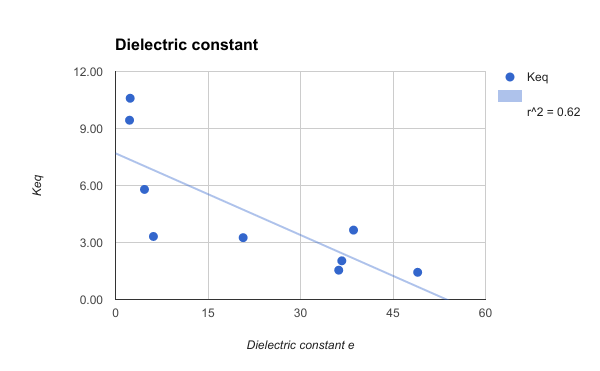
\includegraphics[width=.5\linewidth]{figures/image}
    \caption{Initial condition} 
  \end{minipage}%%
  \begin{minipage}[b]{0.4\linewidth}
    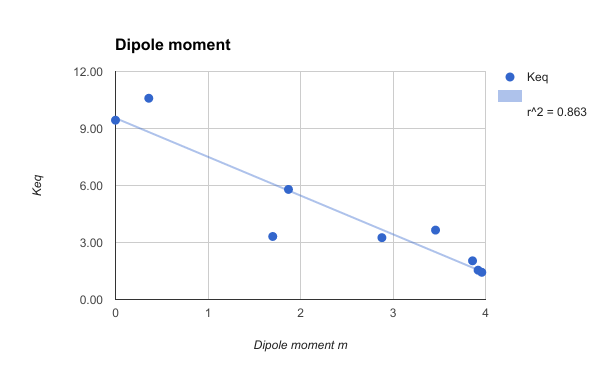
\includegraphics[width=.5\linewidth]{figures/image1}
    \caption{Rupture} 
  \end{minipage}
  \begin{minipage}[b]{0.49\linewidth}
    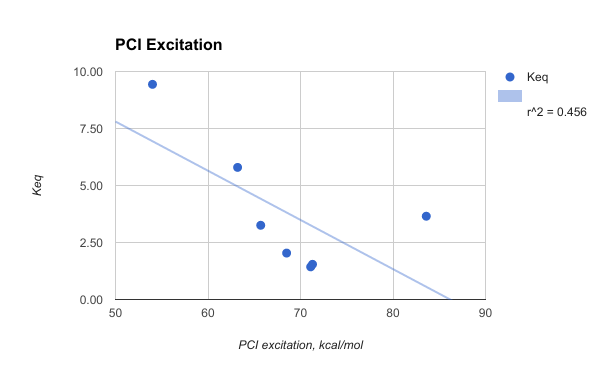
\includegraphics[width=.5\linewidth]{figures/image2}
    \caption{DFT, Initial condition} 
  \end{minipage}%%
  \begin{minipage}[b]{0.49\linewidth}
    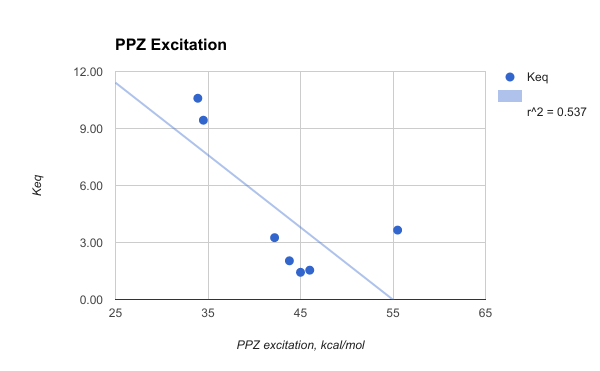
\includegraphics[width=.5\linewidth]{figures/image3}
    \caption{DFT, rupture} 
  \end{minipage} 
\end{figure*}


\begin{@twocolumnfalse}
\section{References}
[1] Experimental Chemistry I: CH 362, OSU Department of Chemistry 2017\\

[2] OSU of Chemistry. 1H NMR Chemical Shifts. http://www.science.oregonstate.edu/~gablek/CH335/Chapter10/ChemicalShift.htm. (Accessed March 22, 2017)\\

[3] University of Washington Department of Chemistry. Dielectric constant table for common solvents. $https://depts.washington.edu/eooptic/linkfiles/dielectric_chart$\%$5B1$\%$5D.pdf$

[4] Computational Chemistry Comparison and Benchmark Database. Experimental Dipoles. http://cccbdb.nist.gov/diplistx.asp
\end{@twocolumnfalse}
\end{document}
